\section*{Results}

\subsection*{Change Point Analysis}
In this analysis, intervals in which Theil-Sen slopes deviate from each other significantly in magnitude, direction, or both are divided by change points denoted by vertical dashed lines of varying color within the dates of 1920 to 2023. Throughout the total time-period, areas of denser data points are indicated by colored dots progressing from hues of light purple at shallower well points to light green at deeper well points. 
\subsubsection*{Ogallala}
In the Ogallala Aquifer, two of these critical points occur in the years 1968 and 1987 and are denoted by a red color in Figure~\ref{fig:OG_CP}. These lines separate three segments, the first with a deepening well depth Theil-Sen slope value of 4.34 ft/yr spanning from 1920 to 1968, the second with a shallowing well depth value of -3.74 ft/yr spanning from 1968 to 1987, and the third with a deepening well depth value of 3.57 ft/yr spanning from 1987 to 2023. The shallowest lognormal mean depth value for the Ogallala Aquifer in the given period was 88.88 feet in the year 1924. 86 years later, in 2010, the deepest lognormal mean value of 504.27 feet was calculated. Since this deepest value, however, the 13 years from 2010 to 2023 exhibit a shallowing trend, though it is important to note that the dataset for this time-period certainly does not accommodate analysis that is rich in accuracy as the number of well points is at its maximum of 38 in 2011 and at a minimum of 3 in 2023. Additionally, each of the colored dots represent one of the 12,572 total data points used to generate this plot.

\begin{figure}[H]
    \centering
    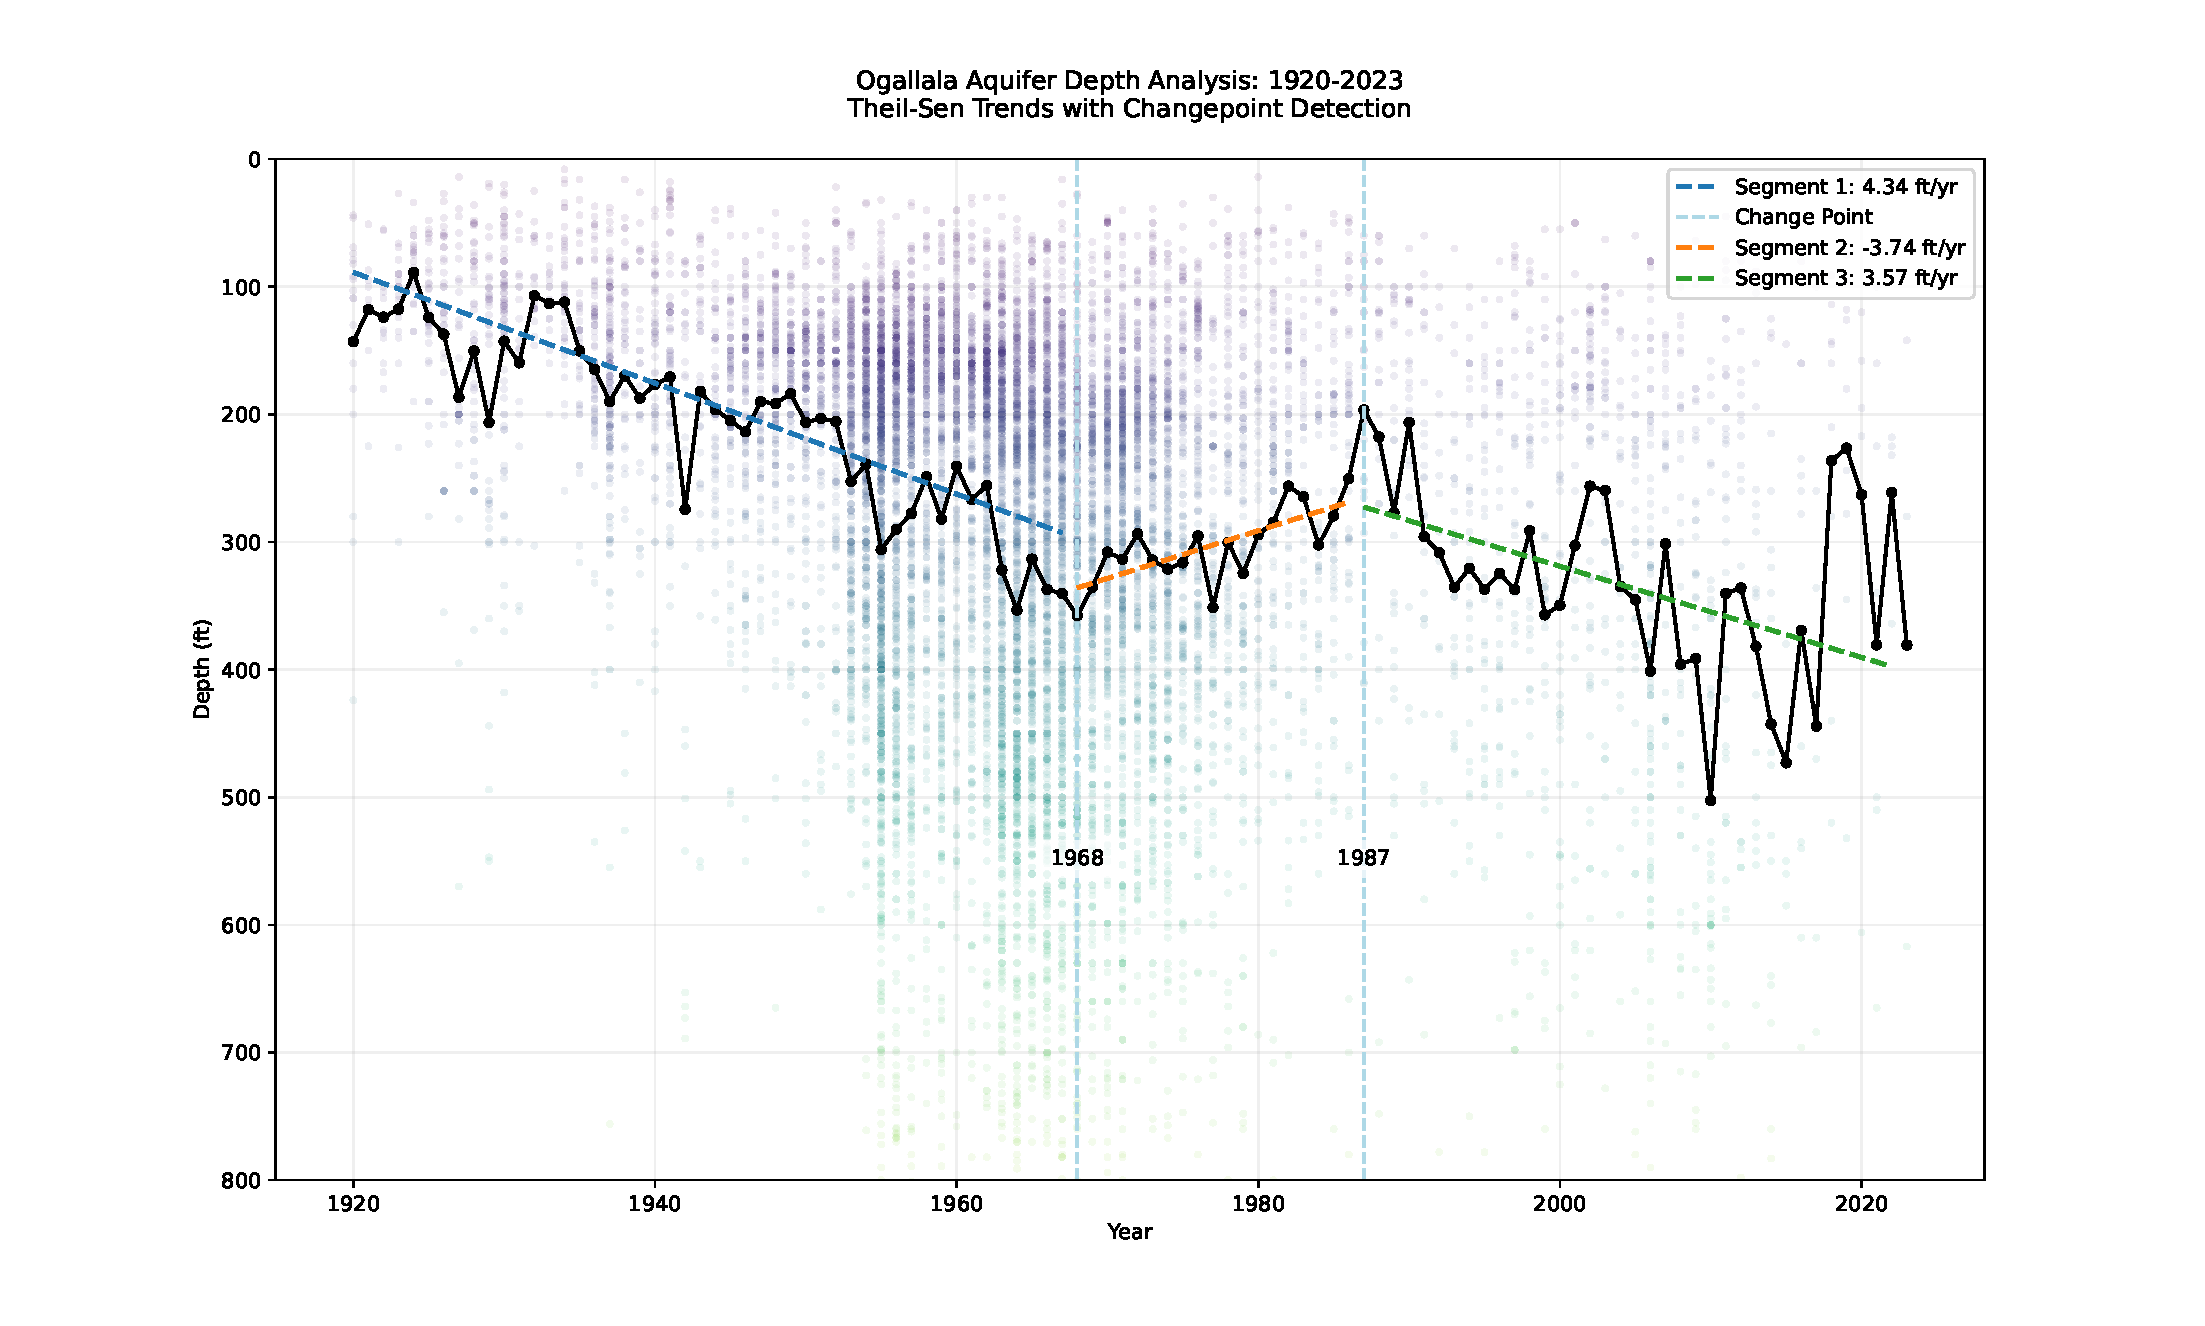
\includegraphics[width=0.75\linewidth]{Figures:Tables/Ogallala/Ogallala_CP.pdf}
    \caption{Enter Caption}
    \label{fig:OG_CP}
\end{figure}
\begin{figure}[H]
    \centering
    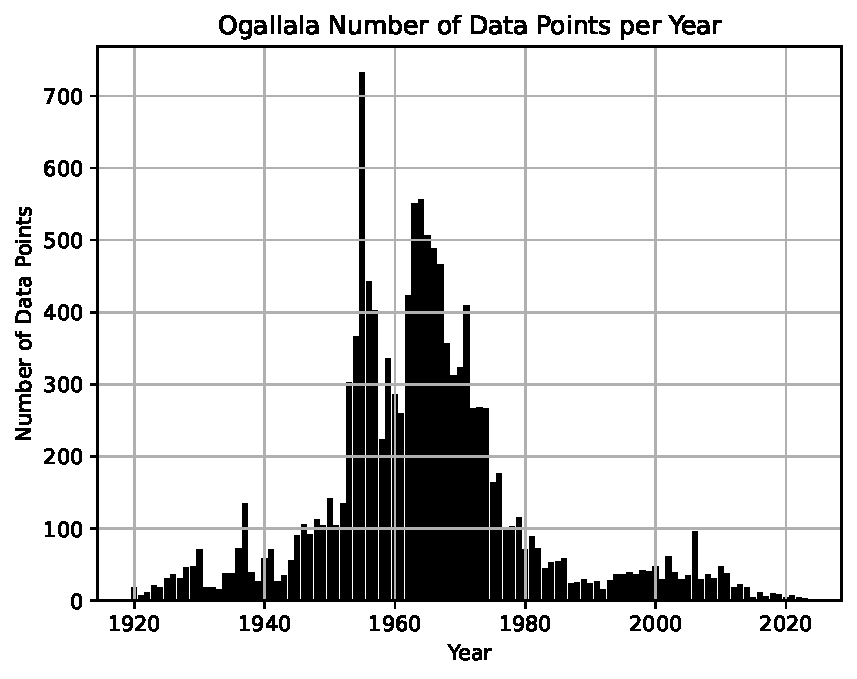
\includegraphics[width=0.5\linewidth]{Figures:Tables/Ogallala/Ogallala_n_values.pdf}
    \caption{Enter Caption}
    \label{fig:OG_n_value}
\end{figure}

\subsubsection*{Edwards (Balcones Fault Zone)}
In the Edwards (Balcones Fault Zone), two critical points were determined to be in the years 1955 and 1980 (Figure~\ref{fig:EBFZ_CP}). The first segment has a deepening Theil-Sen slope of 6.37 ft/yr from the years 1920 to 1955, the second a shallowing slope of -16.36 ft/yr from 1955 to 1980, and the third a shallowing slope of -7.61 ft/yr from 1980 to 2023.  The shallowest lognormal mean throughout the entire period has a value of 322.48 ft in 2019 and the deepest has a value of 1105.34 in 1955. It is also important to note that in 1955 the highest number of wells were drilled, totaling 91 for that year. Similar to the Ogallala aquifer, data points become sparser in later years, as not a single year following 1998 has more than 25 recorded wells. Additionally, it must be noted that this aquifer has a total of 2923 usable well points.
\begin{figure}[H]
    \centering
    \includegraphics[width=0.5\linewidth]{Figures:Tables/EdwardsBFZ/EdwardsBFZ_CP.pdf}
    \caption{Enter Caption}
    \label{fig:EBFZ_CP}
\end{figure}
\begin{figure}[H]
    \centering
    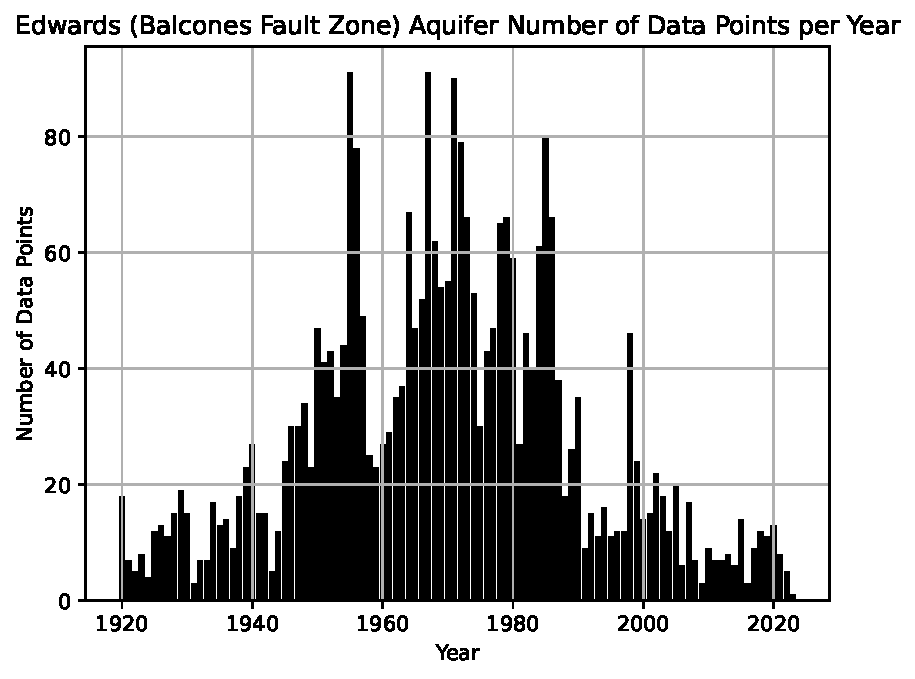
\includegraphics[width=0.5\linewidth]{Figures:Tables/EdwardsBFZ/Edwards (Balcones Fault Zone)_n_values.pdf}
    \caption{Enter Caption}
    \label{fig:EBFZ_n_value}
\end{figure}

\subsubsection*{Edwards-Trinity Plateau}
In the Edwards-Trinity Plateau Aquifer, critical points occur in the years 1968 and 1985 and are light green in color (Figure~\ref{fig:ETP_CP}). The first segment (1920 to 1968) has a deepening Theil-Sen slope of 0.65 ft/yr, the second (1968 to 1985) a shallowing Theil-Sen slope of -4.04 ft/yr, and the third (1985 to 2023) a deepening Theil-Sen slope of 8.54 ft/yr. The shallowest lognormal mean from the period has a value of 135.00 ft and occurs in 2020, while the deepest has a value of 856.48 ft and occurs in 2009. The highest number of wells drilled in one year, though, occurs in 1963 with 231 points, and the lowest number of wells drilled occurs in 2014 with 1 point (Figure~\ref{fig:ETP_n_value}). The total number of well points amounts 5589, and once again, data points become sparser as time goes on, as the mid-to-late 1960’s represent a noticeable divide in the density of points where well points are far denser prior to this relative date.

\begin{figure}[H]
    \centering
    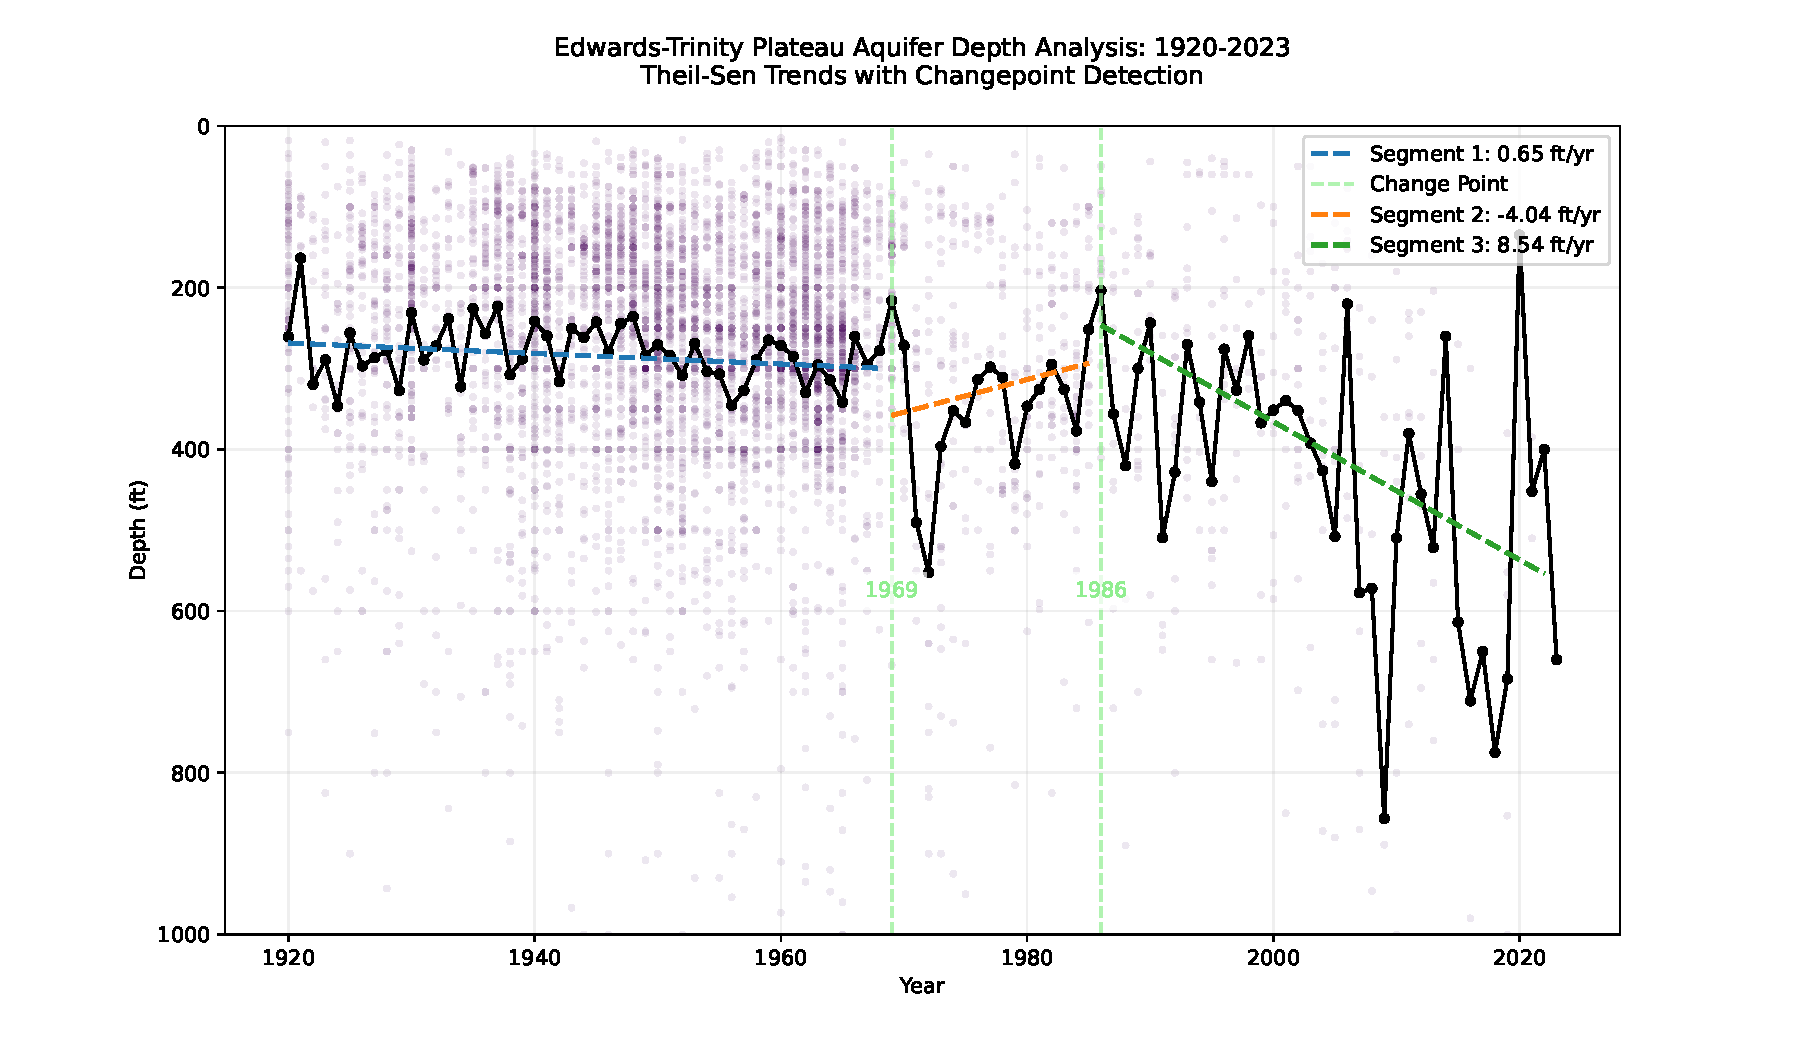
\includegraphics[width=0.5\linewidth]{Figures:Tables/EdwardsTP/EdwardsTP_CP.pdf}
    \caption{Enter Caption}
    \label{fig:ETP_CP}
\end{figure}
\begin{figure}[H]
    \centering
    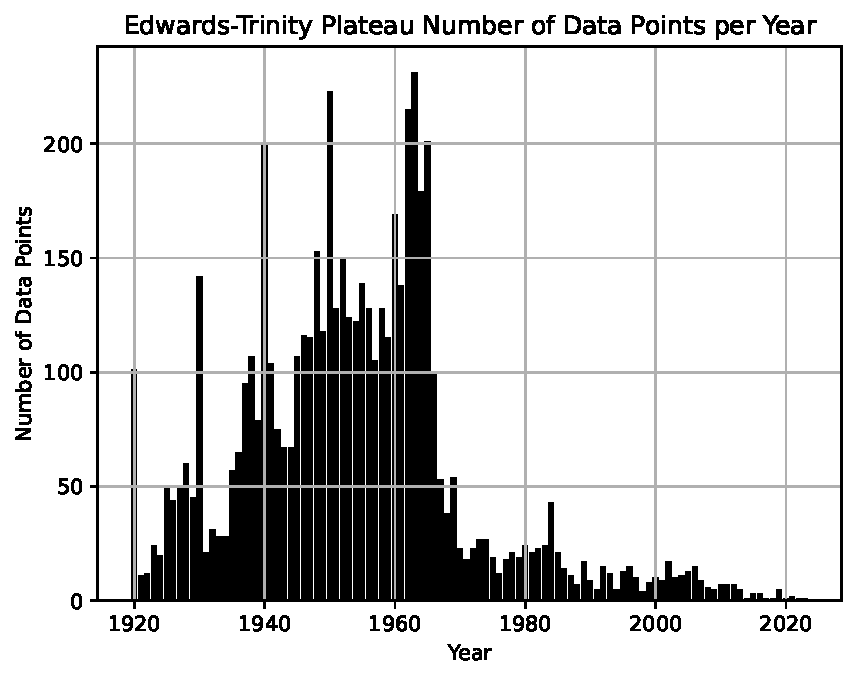
\includegraphics[width=0.5\linewidth]{Figures:Tables/EdwardsTP/Edwards-Trinity Plateau_n_values.pdf}
    \caption{Enter Caption}
    \label{fig:ETP_n_value}
\end{figure}

\subsubsection*{Carrizo-Wilcox}
In the Carrizo-Wilcox Aquifer, there are critical points in red for the years 1944 and 1987 (Figure~\ref{fig:CW_CP}). The first segment (1920 to 1944),  has a deepening Theil-Sen slope value of 6.84 ft/yr, the second (1944 to 1987) with a shallowing slope of -5.78 ft/yr, and the third (1987 to 2023) with a shallowing slope of -1.68 ft/yr. The shallowest lognormal mean value from the time range was 130.41 feet in the year 1933, while the deepest was 1286.71 in the year 1944. The highest number of wells drilled in a year occurred in 1964 with 331 data points, and the lowest number of wells drilled in a year occurred in 2023 with one data point. The total number of data points for the given period in the Carrizo-Wilcox Aquifer is 8020, and values of wells drilled per year create an approximately normal distribution (Figure~\ref{fig:CW_n_value}).

\begin{figure}[H]
    \centering
    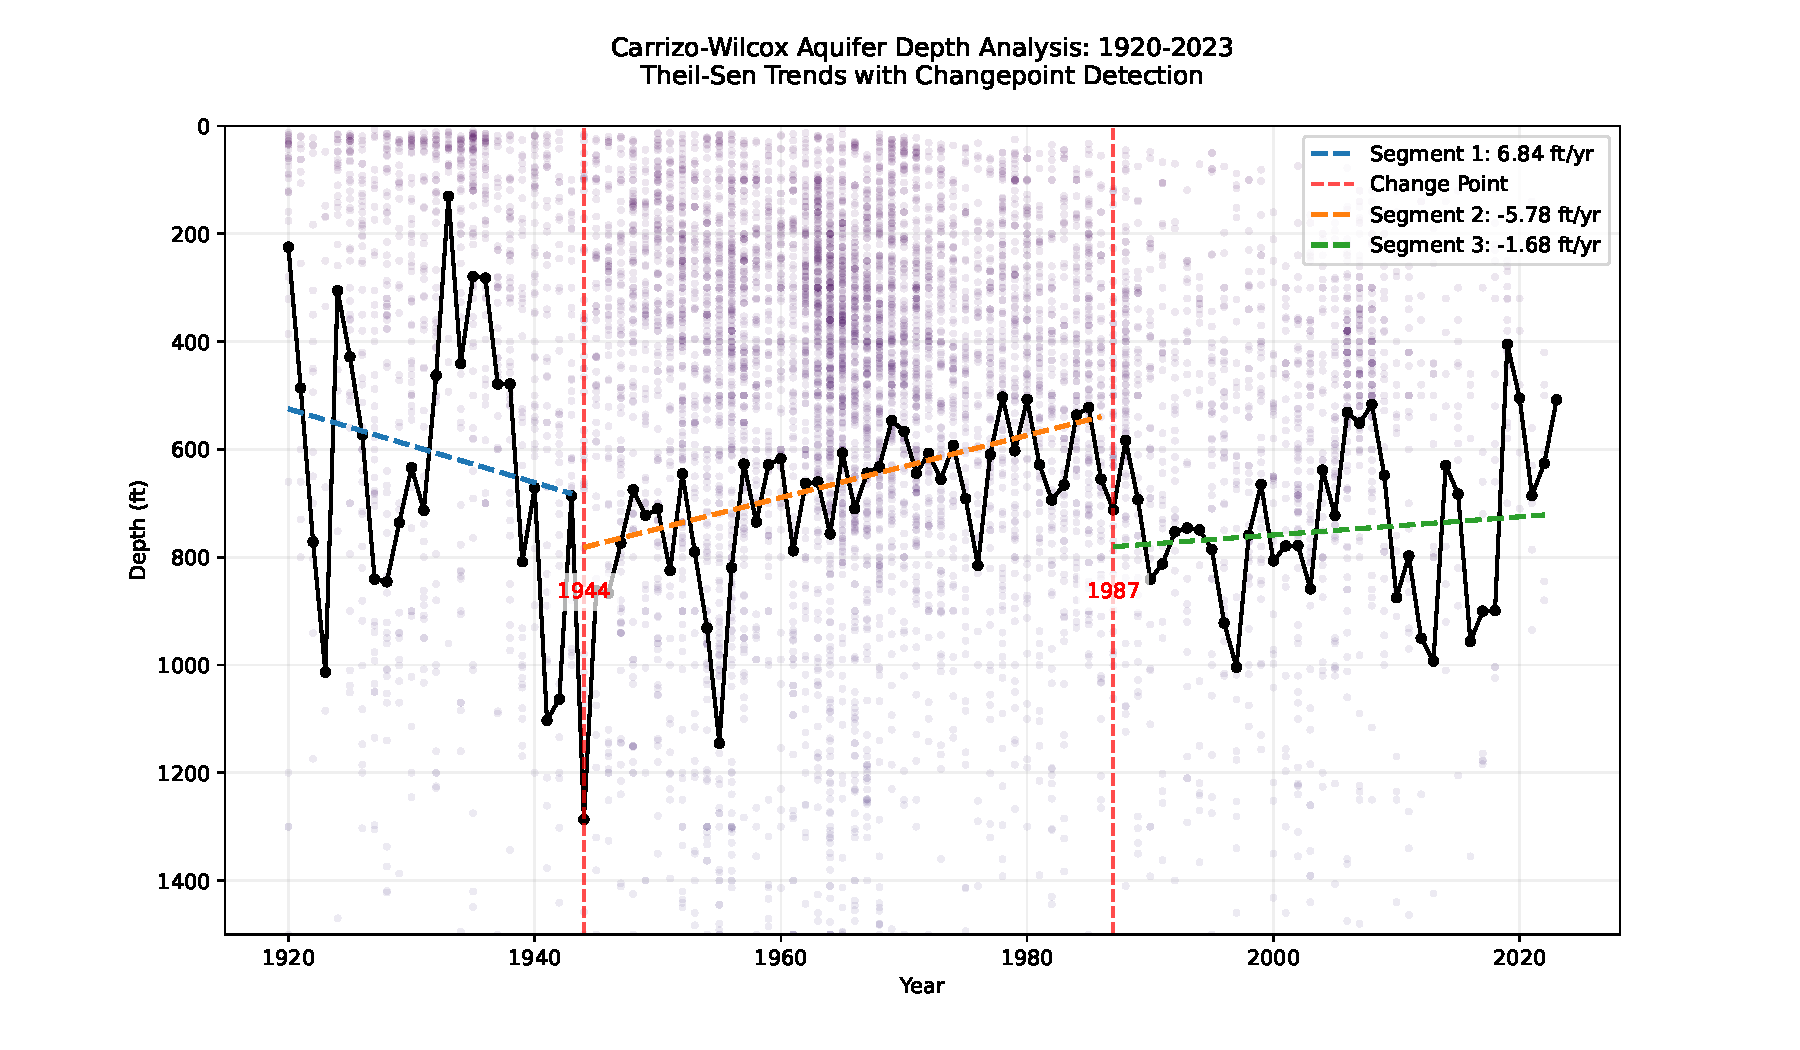
\includegraphics[width=0.5\linewidth]{Figures:Tables/Carrizo_Wilcox/Carrizo-Wilcox_CP.pdf}
    \caption{Enter Caption}
    \label{fig:CW_CP}
\end{figure}

\begin{figure}[H]
    \centering
    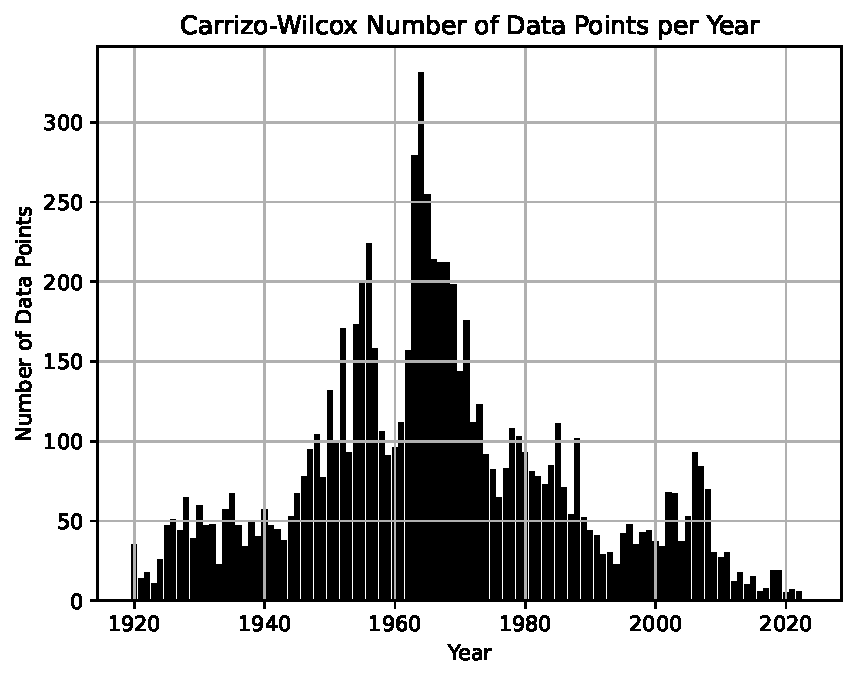
\includegraphics[width=0.5\linewidth]{Figures:Tables/Carrizo_Wilcox/Carrizo-Wilcox_n_values.pdf}
    \caption{Enter Caption}
    \label{fig:CW_n_value}
\end{figure}

\subsubsection*{Gulf Coast}
In the Gulf Coast Aquifer, critical points were determined to be in the years 1949 and 1971 (Figure~\ref{fig:GC_CP}). The first segment (1920 to 1949) has a deepening Theil-Sen slope of 8.03 ft/yr, the second has a shallowing slope of -8.02 ft/yr, and the third has as deepening slope of 1.81 ft/yr. The shallowest lognormal mean through the period was in the year 2022 with a depth value of 205 feet, while the deepest was in the year 2015 with a depth value of 1202.23 feet. The highest number of wells drilled in a year occurs in 1956 with 598 well points and the lowest number of wells drilled in a year occurs in 2022 with 1 well point (Figure~\ref{fig:GC_n_value}). The cumulative number of data points for the Gulf Coast Aquifer in this time period is 19033, reaching the highest number out of the nine major Texas aquifers. The majority of these wells were placed before the 1970s, as seen in the other aquifers (with the exception of the Edwards (Balcones Fault Zone) Aquifer).


\begin{figure}[H]
    \centering
    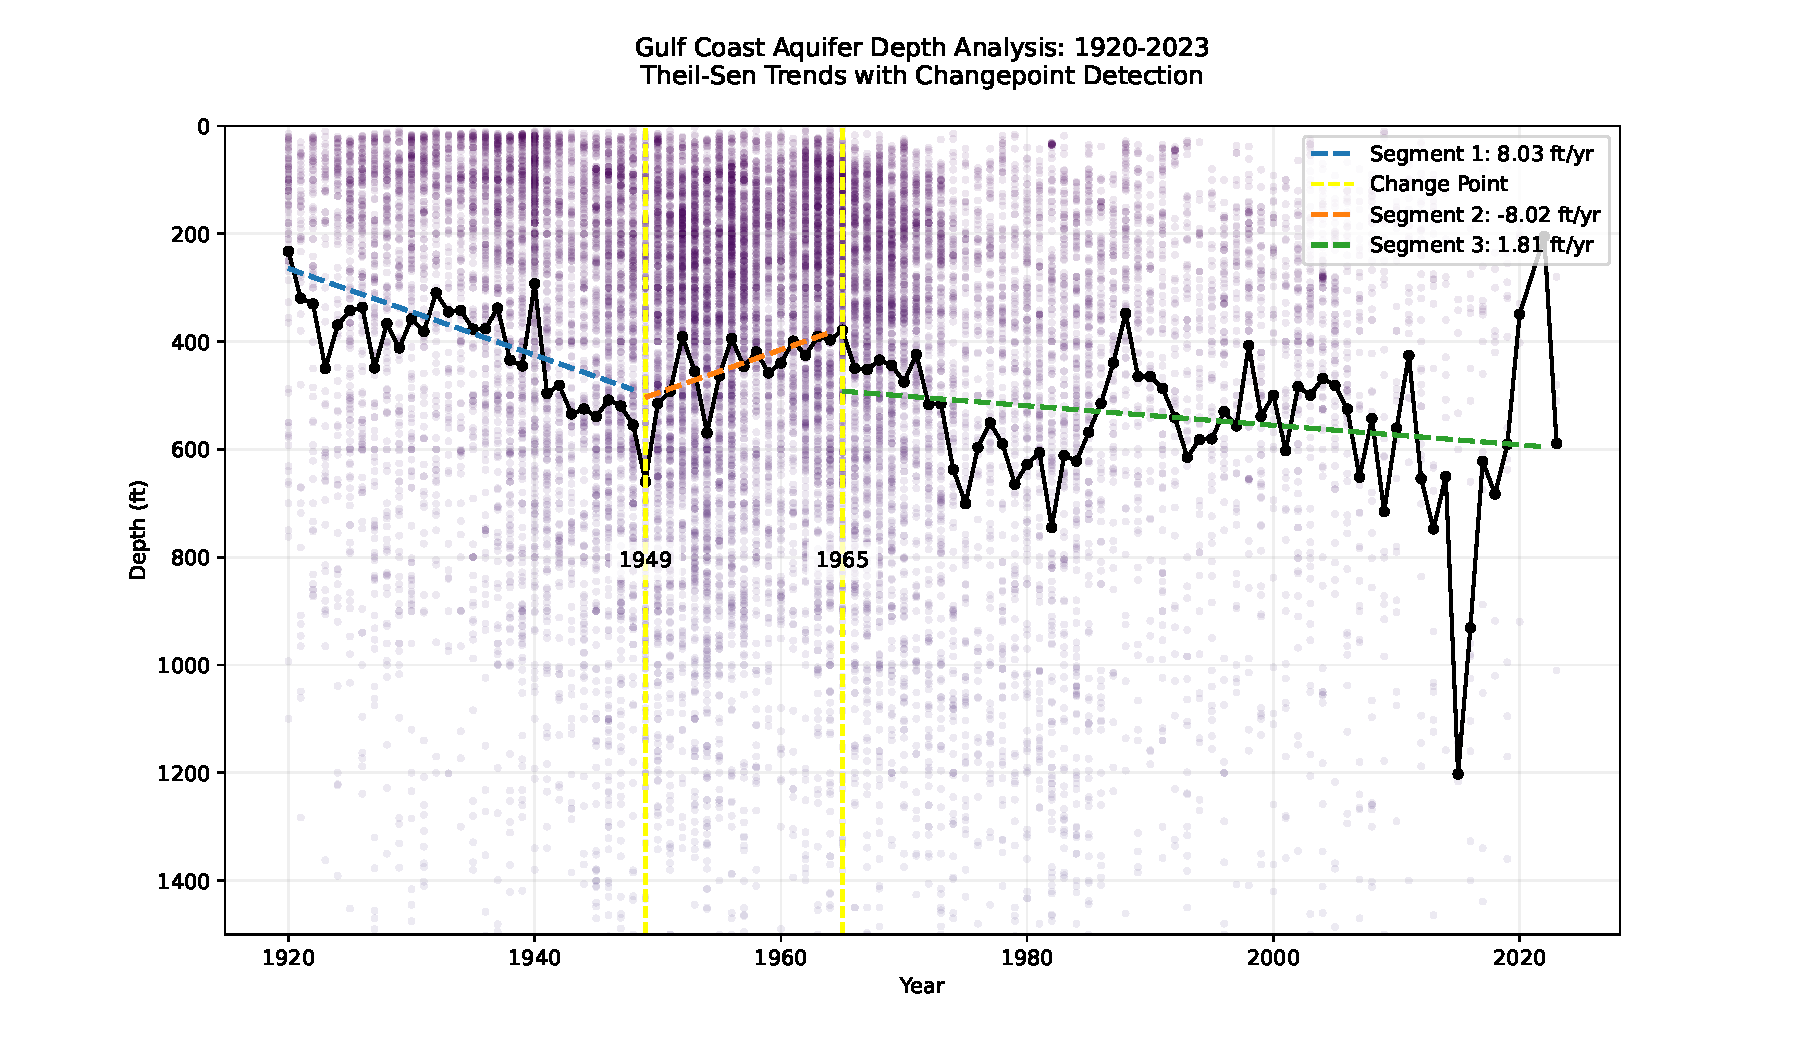
\includegraphics[width=0.5\linewidth]{Figures:Tables/Gulf Coast/GulfCoast_CP.pdf}
    \caption{Enter Caption}
    \label{fig:GC_CP}
\end{figure}

\begin{figure}[H]
    \centering
    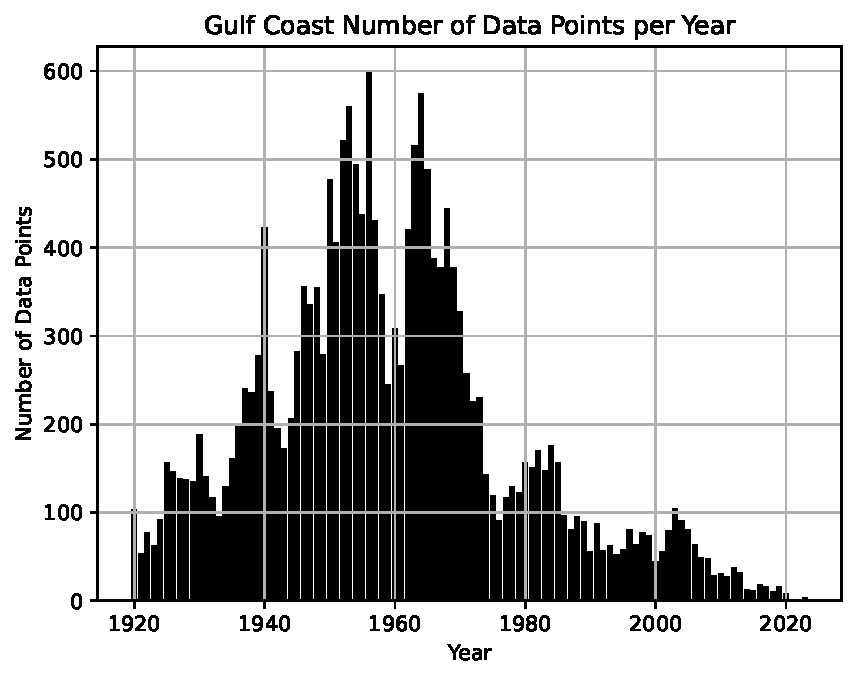
\includegraphics[width=0.5\linewidth]{Figures:Tables/Gulf Coast/Gulf Coast_n_values.pdf}
    \caption{Enter Caption}
    \label{fig:GC_n_value}
\end{figure}

\subsubsection*{Pecos Valley}
In the Pecos Valley Aquifer, two critical points were identified as 1973 and 2007 and are colored orange (Figure~\ref{fig:PV_CP}). The first segment (1920 to 1973) has a deepening Theil-Sen slope of 8.78 ft/yr, the second has a shallowing slope of -5.00 ft/yr, and the third has a deepening slope of 23.91 ft/yr. The shallowest lognormal mean depth value from 1920 to 2023 has a value of 25 feet and occurred in 1922 and the deepest depth has a value of 727.94 and occurred in 1973. Relative to data from other aquifers, the Pecos Valley Aquifer has a far smaller number of total well points, with a value of 1058. Due to this small number of points, several of the later years do not have even one well point.

\begin{figure}[H]
    \centering
    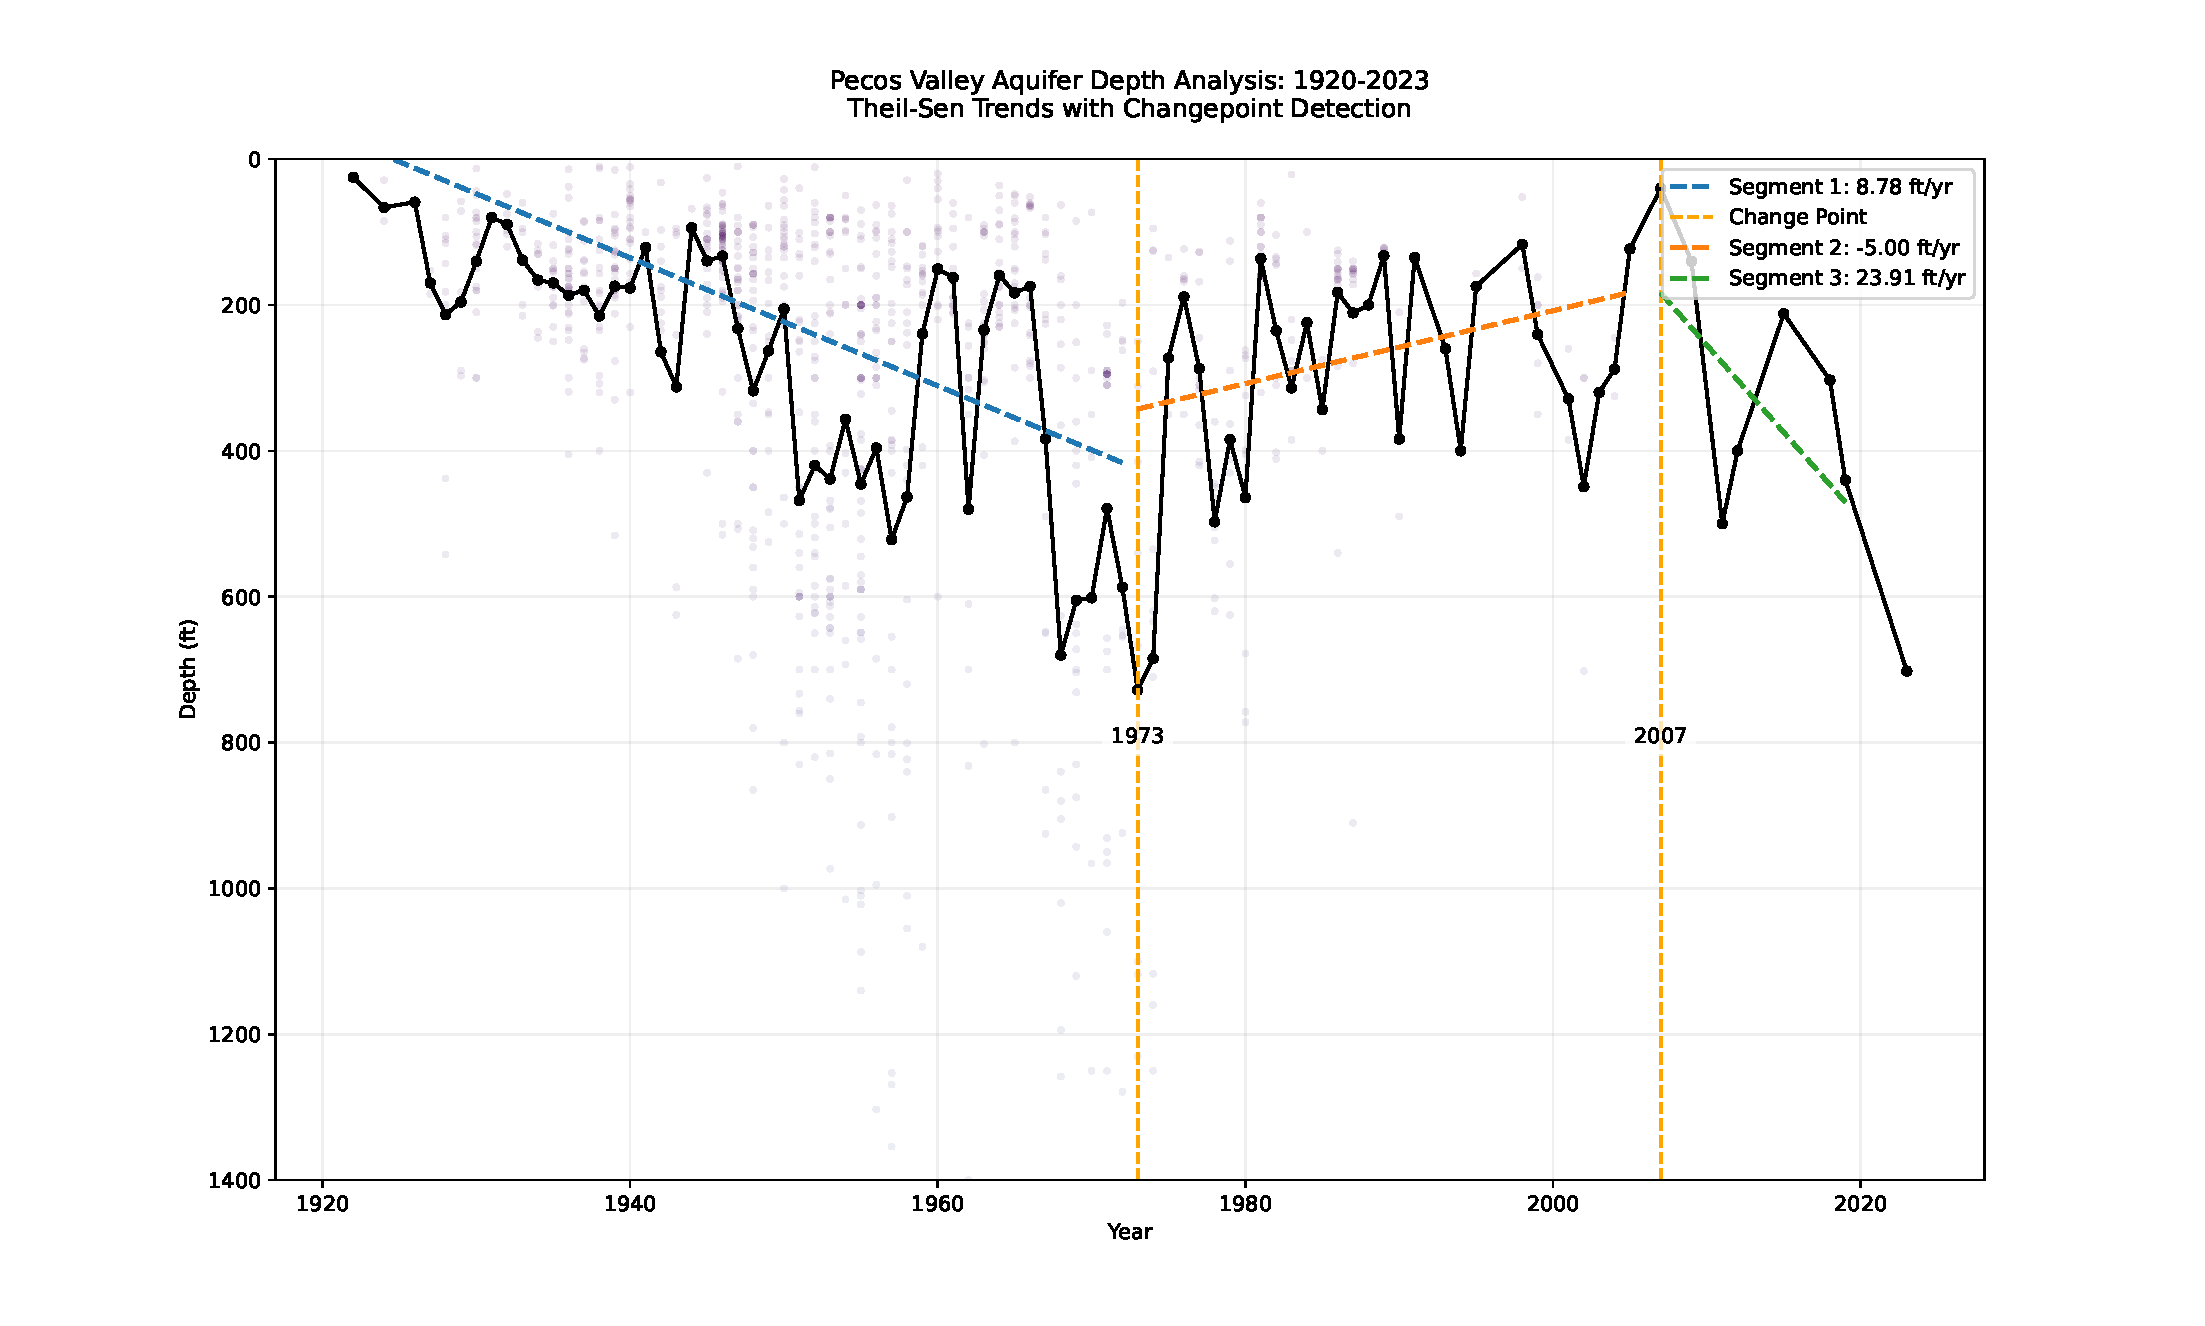
\includegraphics[width=0.5\linewidth]{Figures:Tables/Pecos Valley/PecosValley_CP.pdf}
    \caption{Enter Caption}
    \label{fig:PV_CP}
\end{figure}

\begin{figure}[H]
    \centering
    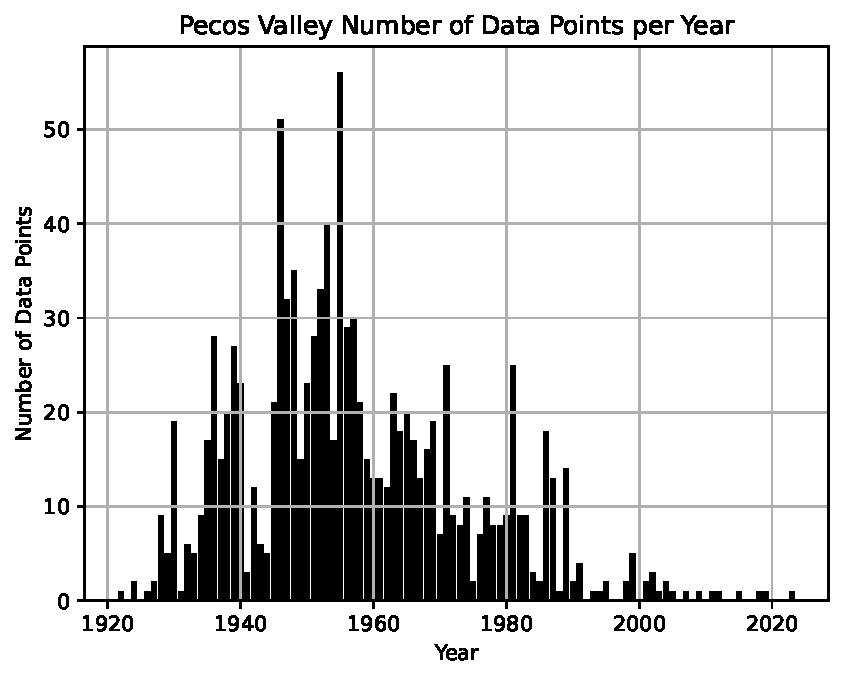
\includegraphics[width=0.5\linewidth]{Figures:Tables/Pecos Valley/Pecos Valley_n_values.pdf}
    \caption{Enter Caption}
    \label{fig:PV_n_value}
\end{figure}

\subsubsection*{Seymour}
The Seymour Aquifer has a singular critical point in the year 1976 that is brown in color (Figure~\ref{fig:SM_CP}). The first segment (1920 to 1976) has as deepening Theil-Sen slope of 0.27 ft/yr that then gives way to the second segment (1976 to 2013) with a deepening slope of 2.04 ft/yr. The years after 2013 are not accounted for in this chart because there is only one more data point, which is in 2016, and thus there is not enough data for the Theil-Sen regression to continue. The shallowest lognormal mean for this period occurs in 1939 and has a value of 30.49 feet, while the deepest occurs in 2011 and has a value of 162.00 feet. The highest number of wells drilled in a year was in 1956 with 421 data points and the lowest number was 0, of which a multitude of years after 1980 are guilty of (Figure~\ref{fig:SM_n_value})

\begin{figure}[H]
    \centering
    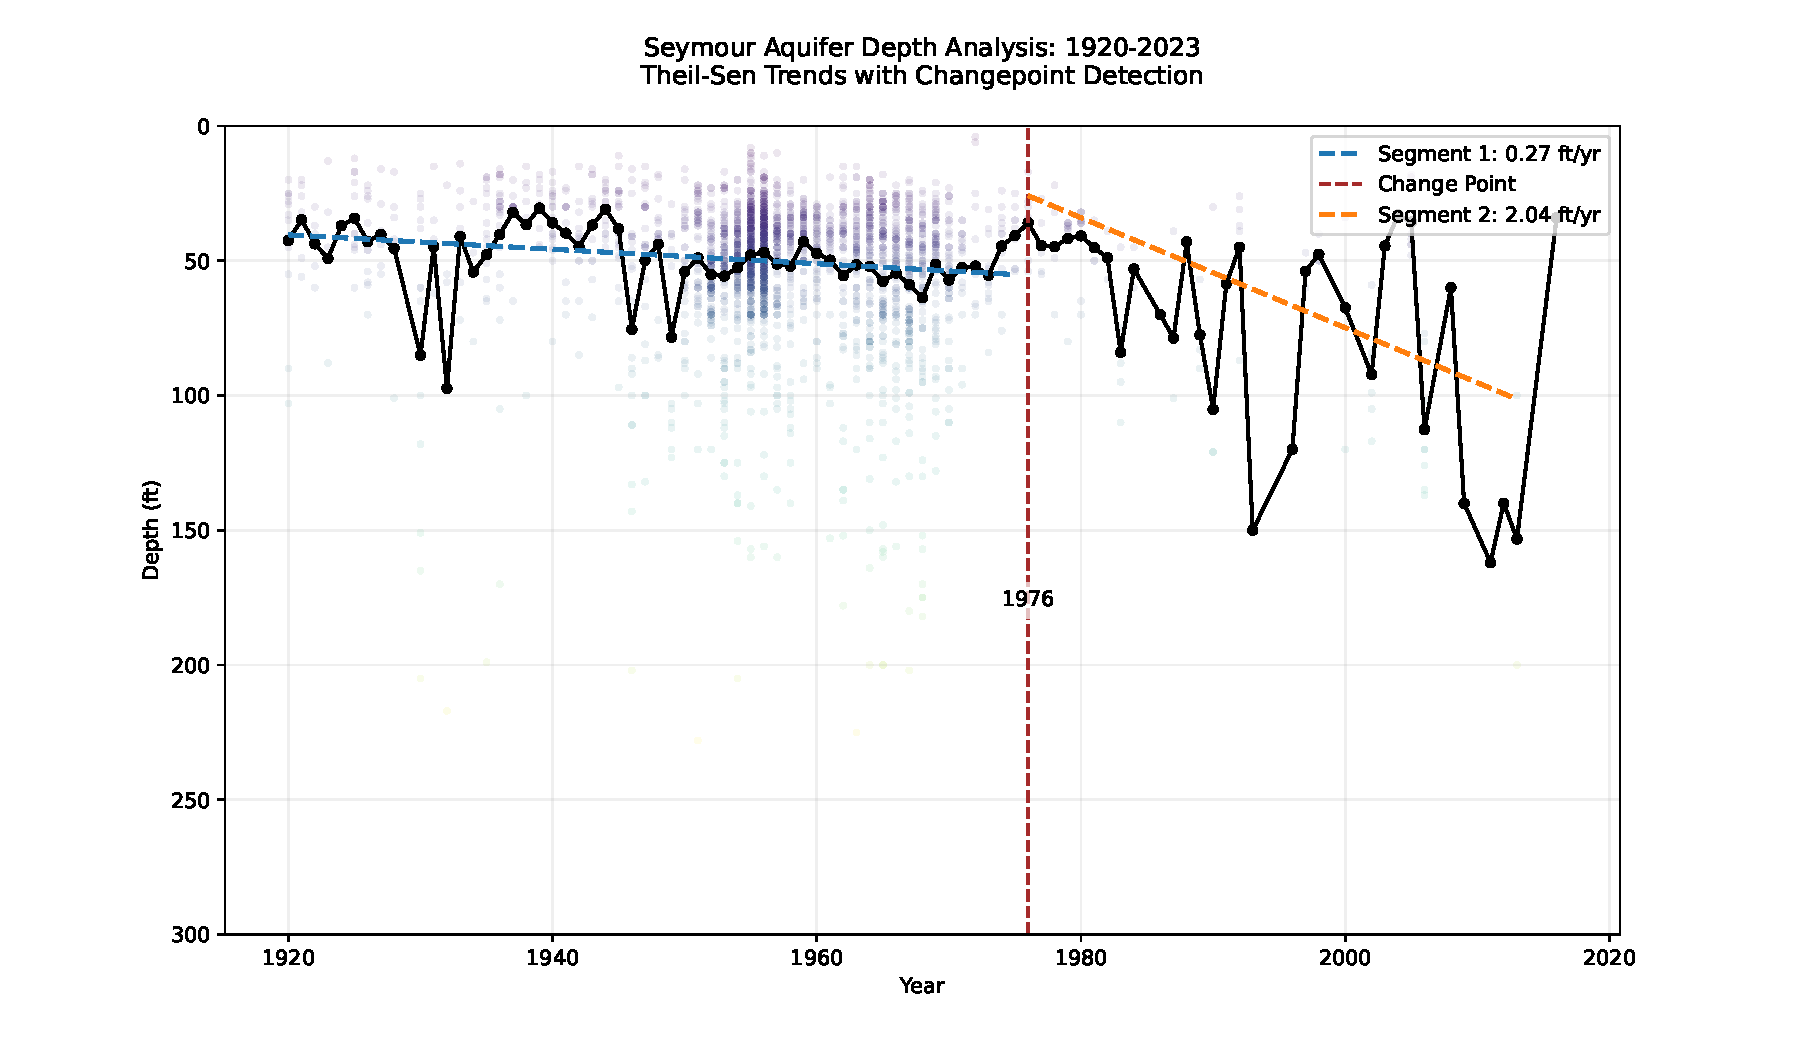
\includegraphics[width=0.5\linewidth]{Figures:Tables/Seymour/Seymour_CP.pdf}
    \caption{Enter Caption}
    \label{fig:SM_CP}
\end{figure}


\begin{figure}[H]
    \centering
    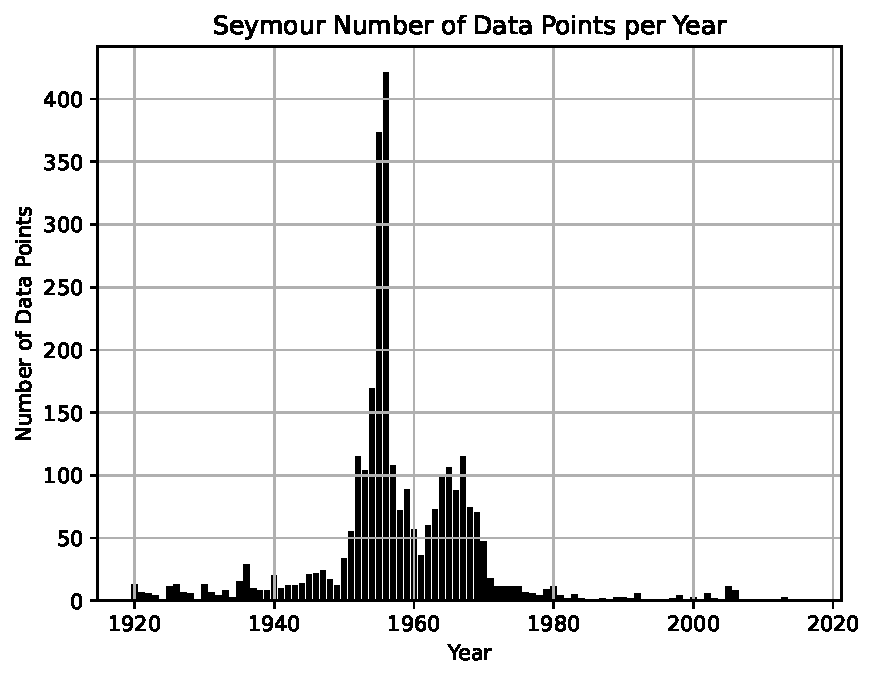
\includegraphics[width=0.5\linewidth]{Figures:Tables/Seymour/Seymour_n_values.pdf}
    \caption{Enter Caption}
    \label{fig:SM_n_value}
\end{figure}


\subsubsection*{Trinity}
The Trinity Aquifer has three critical points, colored green, that occur in the years 1958, 1969, and 2003 (Figure~\ref{fig:TR_CP}). The first segment (1920 to 1958) has a deepening Theil-Sen slope of 5.48 ft/yr, the second (1958 to 1969) has a shallowing slope of -46.36 ft/yr, the third (1969 to 2003) has a deepening slope of 5.83 ft/yr, and the fourth (2003 to 2023) has a shallowing slope of -7.79 ft/yr. The shallowest lognormal mean value of 215.77 feet is in 1966 and the deepest value of 1386.66 is in 1924. The highest number of wells drilled in one year is in 1969 with a value of 500, while the lowest is in 1921 with 13 points (Figure~\ref{fig:TR_n_value}). The total number of well points amounts to 10544 and follows a normal distribution with the amount of wells drilled peaking in the mid-to-late 1960’s. 

\begin{figure}[H]
    \centering
    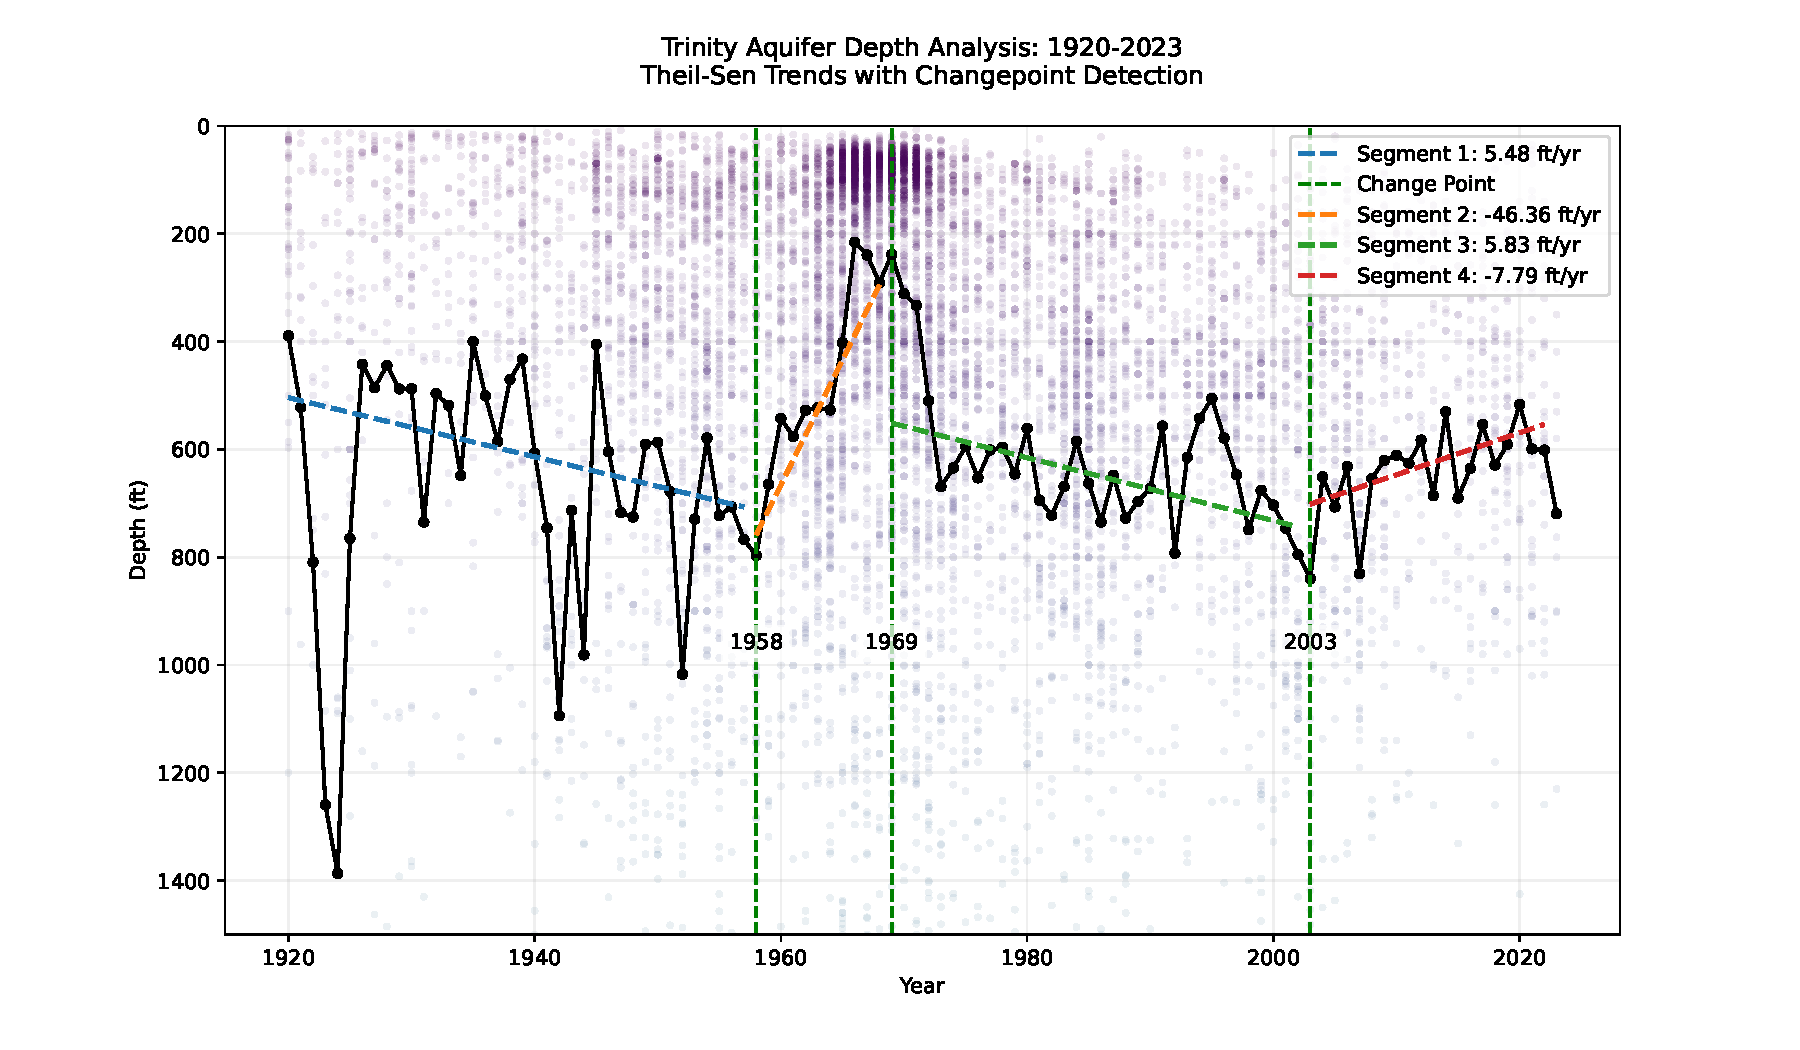
\includegraphics[width=0.5\linewidth]{Figures:Tables/Trinity/Trinity_CP.pdf}
    \caption{Enter Caption}
    \label{fig:TR_CP}
\end{figure}

\begin{figure}[H]
    \centering
    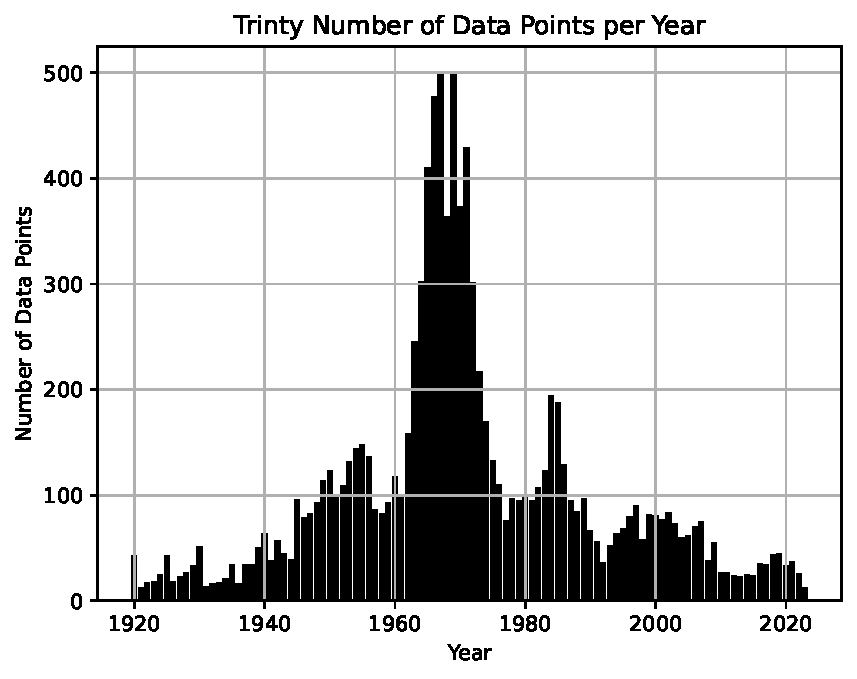
\includegraphics[width=0.5\linewidth]{Figures:Tables/Trinity/Trinity_n_values.pdf}
    \caption{Enter Caption}
    \label{fig:TR_n_value}
\end{figure}

\subsubsection*{Hueco-Mesilla Basin}
The Hueco-Mesilla Basin Aquifer has one critical point in the year 1950 colored in pink (Figure~\ref{fig:HM_CP}). The first segment (1920 to 1950) has a shallowing Theil-Sen slope of -8.28 ft/yr and the second segment (1950 to 2021) has a deepening slope of 2.84 ft/yr. The shallowest lognormal mean depth value from the given time interval has a depth of 234.27 feet and occurs in 2000, while the deepest has a depth of 971.74 feet and occurs in 1959. This basin has the lowest cumulative amount of well points with a total of 985 usable well values, with the most wells drilled in a year being 41 in 1953 and the lowest being none in multiple years, particularly after the year 2006 (Figure~\ref{fig:HM_n_value}). The distribution of wells drilled per year is far more uniform in this aquifer than in others, though it does seem to exhibit a slight tendency towards a normal distribution.

\begin{figure}[H]
    \centering
    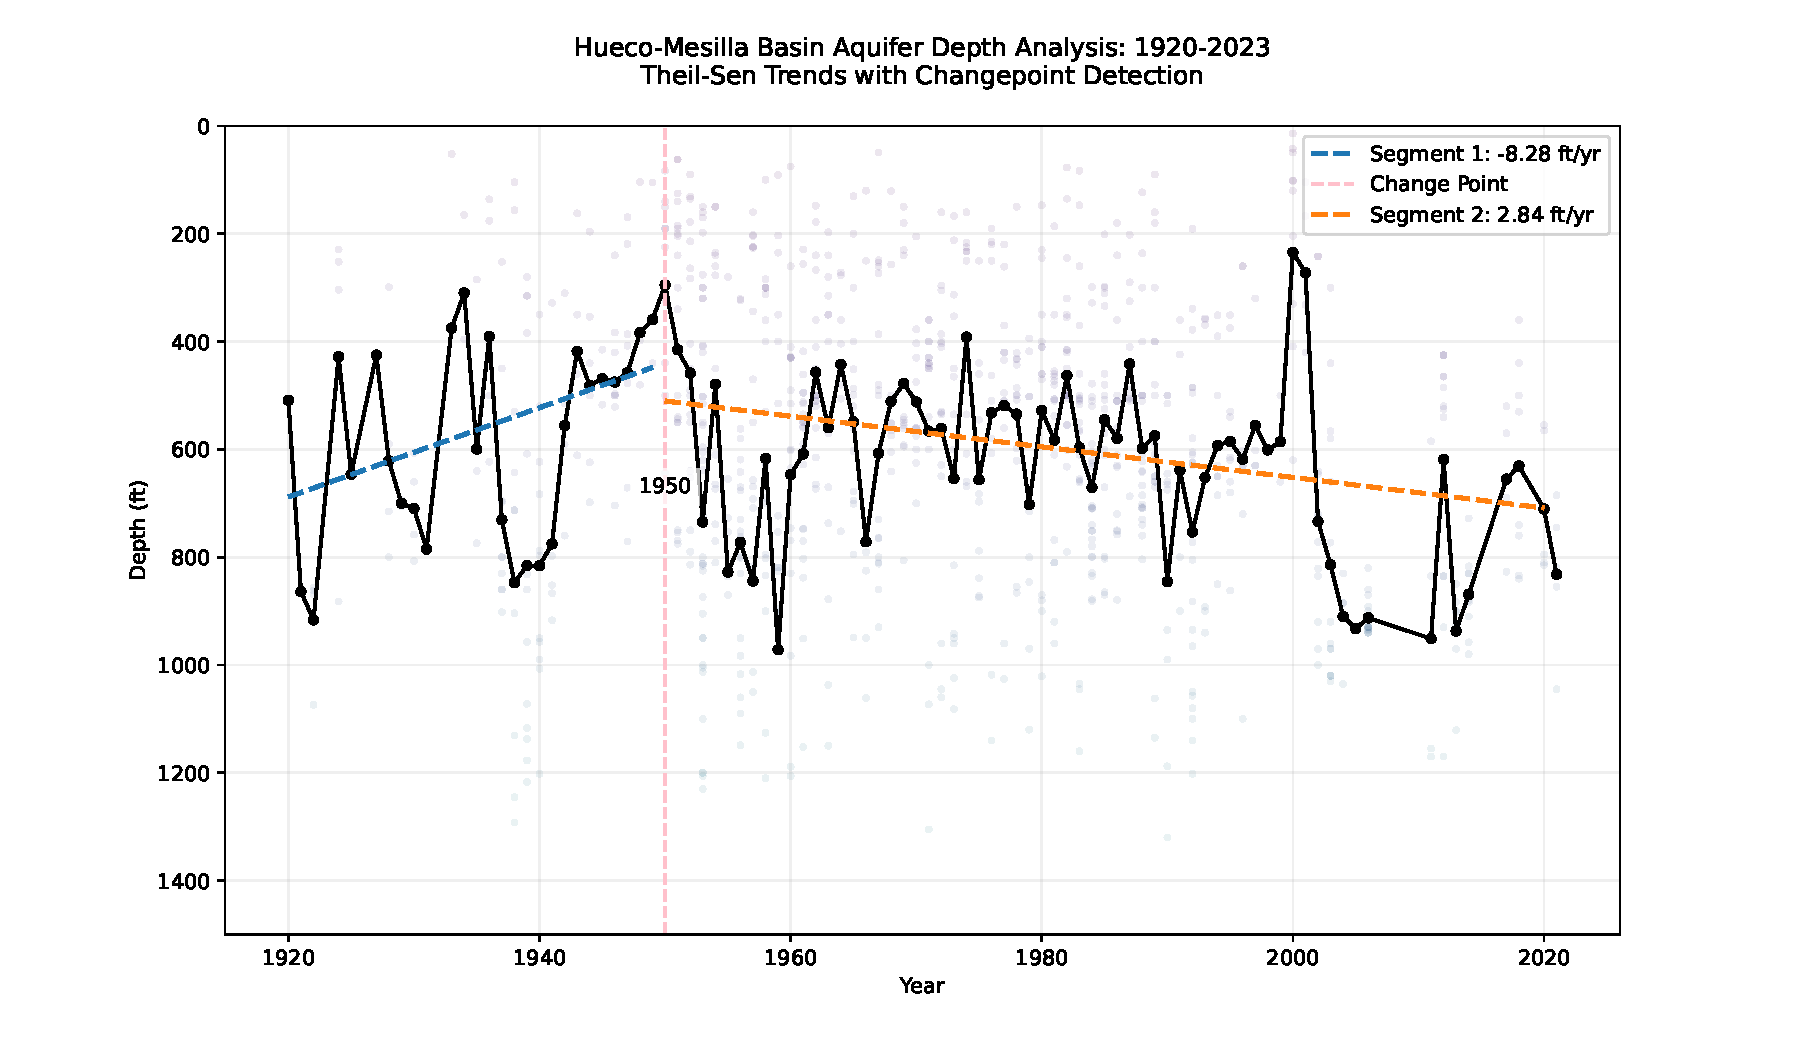
\includegraphics[width=0.5\linewidth]{Figures:Tables/Hueco-Mesilla Basin/HMB_CP.pdf}
    \caption{Enter Caption}
    \label{HM_CP}
\end{figure}

\begin{figure}[H]
    \centering
    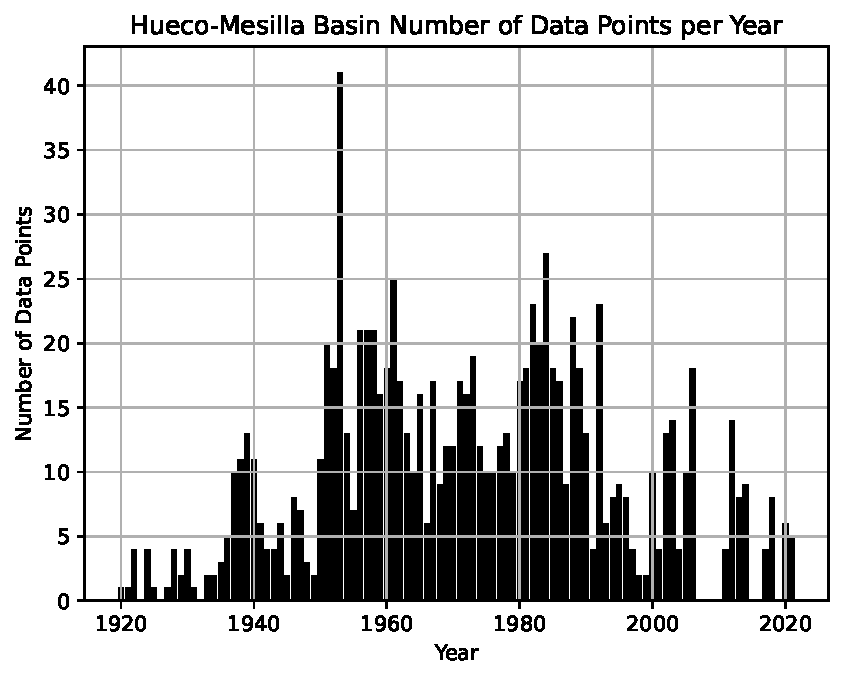
\includegraphics[width=0.5\linewidth]{Figures:Tables/Hueco-Mesilla Basin/Hueco-Mesilla Basin_n_values.pdf}
    \caption{Enter Caption}
    \label{fig:HM_n_value}
\end{figure}
